\subsubsection{Scenarios}

\quad \textbf{User creates an account on the platform}\\ 
Two main users of the platform have to create an account (companies and students). Company has to provide all the information relevant for the company, while student uploads their CV and other relevant information to create a profile that showcases their skills and experiences.\\

\textbf{Company creates an internship advertisement}\\
A company access the platform using their credentials and selects an option to create an internship advertisement. After opening the page for creation of the advertisement, the platform requires detailed internship description, specifying required skills, project descriptions, offered benefits, and application instructions. Also, the company must define how will the selection process look like (e.g. if there will be more then one interview, questionnaire or more than one round of selection process)  \\

\textbf{Company manages internship advertisements}\\
Anytime, a company has an option on the platform to manage active internship advertisements. A company has possibility to update or remove an existing advertisement, ensuring it reflects the latest requirements or availability.\\

\textbf{Student searches and applies for internship opportunities }\\
A student after logging in with his credentials on the platform, the home page is populated with the active internship advertisements which one can browse, filtering by location, required skills, or other criteria. After finding and selecting appropriate internship, the platform opens page with the detailed description, requirements and other information about the internship. Student has an option to apply for the selected internship.\\

\textbf{Company reviews student applications}\\
A company, on their profile can view student applications for every active internship advertisement. The company can evaluate every student's suitability based on uploaded CV, skills and preferences. The platform provides an option for the applied students to accept and continue with the selection process as the company has chosen in the creation of the advertisement, or reject student if they believe they are not right fit for the company. After the acceptance of the certain students, the company has an option to send them questionnaire. \\

\textbf{Student participates in the selection process}\\
After the company selects the student to continue with the selection process, the student receives a notification and has an option to complete a questionnaire provided by a company. The student submits filled questionnaire and waits for the company to send him an invitation for the interview. During the selection process, student has an option to see his progress and all the rounds he has to pass in order to finish the selection process (e.g., questionnaire completed, interview completed).\\

\textbf{User provides feedback on the platform}\\
After the internship concludes, users will get a feedback questionnaire from the platform in order to collect statistical data and improve the recommendation system. The company has to provide feedback about the student’s performance and the platform’s usefulness, while the student has to give some insights about the internship and the company that he worked for.\\

\textbf{The platform recommends internships to students}\\
The recommendation system integrated in the platform recommends internships to the student based on his projects, CV and relevant data that the student uploaded when creating an account. The recommendation system analyzes a student’s profile and suggests internships that match their skills, experiences, and preferences. The recommendation system utilizes simple keyword searching in order to match the internships that could be related to the student's portfolio. \\

\textbf{User submits a complaint to the platform}\\\
During the internship, both the student and the company can file a complaint about issues that can arise. Both users have an option on the platform to file a complaint on the active or completed internship. The platform handles the complaint further. \\

\textbf{University reviews and handles complaints}\\
After the complaint has been filled, the university gets a notification about an active complaint request with all the information that user mentioned. The university communicates with the company and the student to resolve the issue, potentially leading to corrective actions or termination of the internship. If the university decides that the company has not met the benefits and requirements that were mentioned in the internship advertisement, the university can request from the platform to forbid internships from that company to its students.\\

\textbf{University monitors internship progress}\\
The university has an option to monitor the internship progress through feedback related to ongoing internships to ensure compliance with academic and ethical standards. Also, the university has an option to monitor an active internship in order to assign the points to the student in the case of an obligatory internship. \\

%\textbf{Student receives notifications for new internships}\\
%The platform notifies a student about newly added internships that match their profile and preferences.\\

%\textbf{Company conducts interviews via the platform}\\
%A company schedules and conducts interviews with candidates through integrated video calls or other system-%supported methods.\\

%\textbf{Company finalizes candidate selection}\\
%A company selects the most suitable candidate(s) for the internship and sends a confirmation through the platform.\\

\subsubsection{Domain class diagram}

\quad The domain class diagram for the S\&C platform is presented in figure 1 It is designed to represent all major entities and relationships described in the scenarios. The User class serves as a base class for Student, Company, and University which extend it. It encapsulates common attributes. Each subclass adds specific details needed for each role, such as CV and preferences for students, companyName and description for companies, and universityName for universities. Other key classes include InternshipAdvertisement for managing detailed internship postings, InternshipApplication for tracking application statuses, and Complaint for handling issues raised by users. Additional classes like Recommendation and Feedback enhance platform functionality by supporting personalized internship suggestions and collecting user feedback. \\

The relationships between these classes reflect real-world interactions. For instance, companies create and manage InternshipAdvertisement objects, which are linked to multiple InternshipApplication objects submitted by students. The Recommendation class associates student profiles with internships using criteria (e.g. skills and preferences). Both students and companies can provide Feedback about internships and file Complaint objects for university review. Universities handle complaints, monitor internships through the InternshipMonitoring class, and ensure compliance with academic standards.

\begin{figure}[H]
	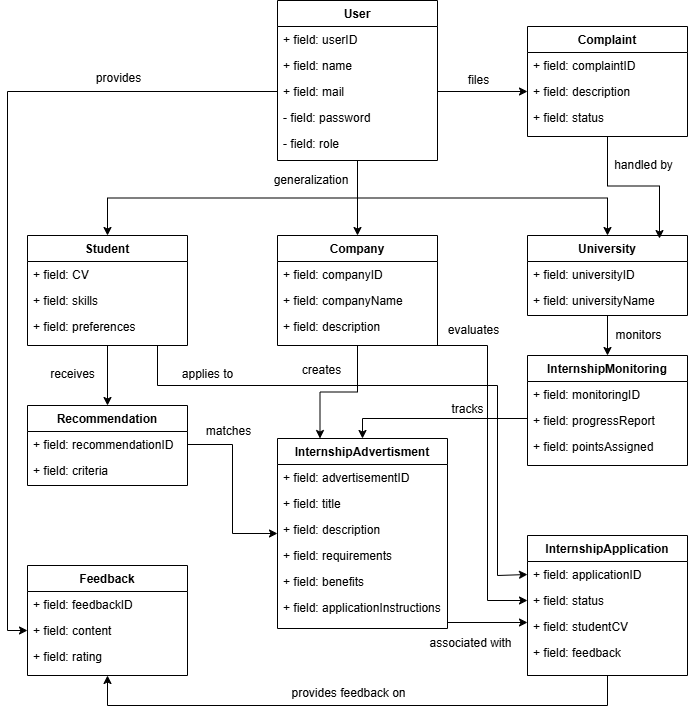
\includegraphics[width=\textwidth,height=\textheight,keepaspectratio]{RASD-Latex/assets/UML - diagram.png}
	\caption{Domain class diagram}
	\label{fig:DataRequest}
\end{figure}


%These relationships and associations provide all the functionalities on the platform, from internship advertisement creation to application management, selection processes, and complaint resolution. \\

%This design emphasizes scalability, maintainability, and data integrity. Its modular structure supports future feature expansion, such as additional user roles or advanced recommendation algorithms. By separating responsibilities among students, companies, and universities, the system ensures clarity and efficiency. Strong associations between classes enforce data consistency, while role-specific features improve usability for all stakeholders. Overall, the diagram provides a comprehensive foundation for implementing the S\&C platform.


\subsubsection{State diagrams}

\quad This section is going to visually present lifecycle of different components on the platform using state diagrams. Following state diagrams are covering management of internship advertisement, internship application and complaint handling. \\

\newpage
\textbf{Internship advertisement management}\\
\begin{figure}[H]
	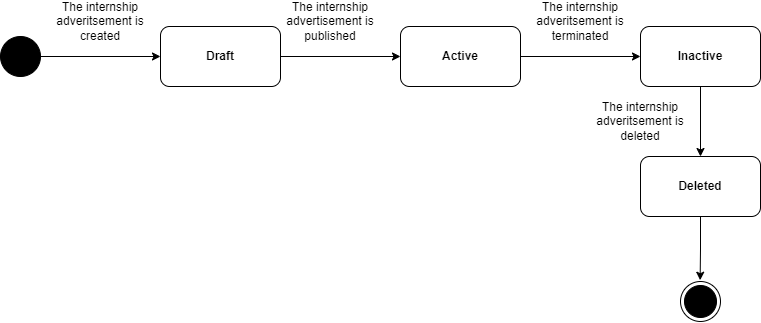
\includegraphics[width=\textwidth,height=\textheight,keepaspectratio]{RASD-Latex/assets/state_diagram.png}
	\caption{Internship advertisement state diagram}
	\label{fig:DataRequest}
\end{figure}

This diagram represents the lifecycle of an internship advertisement on the platform, focusing on states like \textit{Draft}, \textit{Active}, \textit{Inactive}, and \textit{Deleted}. Internship advertisement lifecycle starts from the state \textit{Draft}. This is the initial state when a company starts creating an internship advertisement until it is published. Companies can add details such as required skills, project descriptions, and selection processes. Once the advertisement is finalized and submitted, it transitions to the \textit{Active} state. Active advertisements are visible to students, allowing them to search and apply. The advertisement can be marked as inactive by the company if it's no longer available or requires updates. Inactive advertisements are not visible to students. If the advertisement is no longer needed, it transitions to the \textit{Deleted} state. Deleted advertisements are permanently removed from the platform. Transitions between these states occur based on user actions.\\

\newpage
\textbf{Internship application management}\\
\begin{figure}[H]
	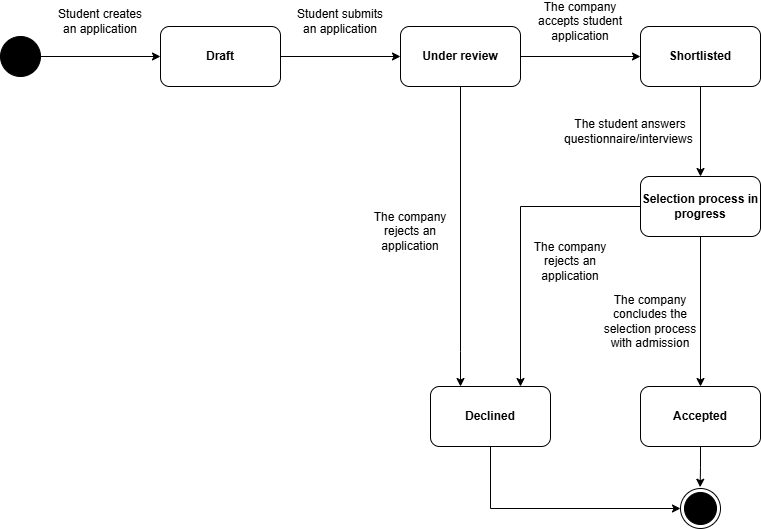
\includegraphics[width=\textwidth,height=\textheight,keepaspectratio]{RASD-Latex/assets/state_diagram_2.png}
	\caption{Internship application state diagram}
	\label{fig:DataRequest}
\end{figure}

Application and selection process for students and companies are showed in the state diagram above (figure 3). After a student applies for an internship, their application enters the \textit{Under Review} state. The company evaluates the application based on the CV and profile. If the student’s application meets the company’s criteria, it transitions to the \textit{Shortlisted} state. The student is notified of their progress. After shortlisting, the selection process begins. This could involve questionnaires, interviews, or other methods defined by the company. The platform keeps track of the student's progress through each stage. If the student is not a fit, their application transitions to the \textit{Declined} state with the reason for that decision indicated by the company. The student is notified of the rejection. On the other hand, if the student successfully completes all selection stages, their application moves to the \textit{Accepted} state. This indicates that the student has secured the internship. \\

\newpage
\textbf{Complaint management}\\
\begin{figure}[H]
	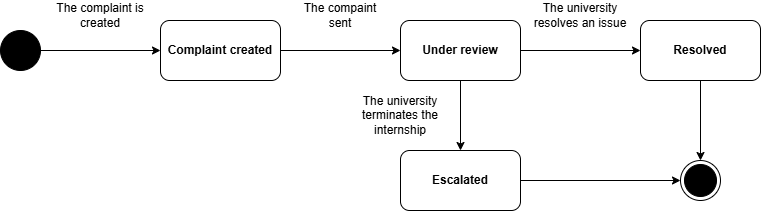
\includegraphics[width=\textwidth,height=\textheight,keepaspectratio]{RASD-Latex/assets/state_diagram_3.png}
	\caption{Complaint handling state diagram}
	\label{fig:DataRequest}
\end{figure}

The complaint process starts when a user (student or company) creates a complaint. The complaint moves to the state \textit{Complaint created}. Immediately, the next state \textit{Under review} is active. In that state, the university begins the review process. In this state, the university evaluates the complaint, gathering information from involved parties (e.g., students, companies, or both). If the issue cannot be resolved, the university has an option to terminate the internship and in that case state is \textit{Escalated}. Whereas, if the university successfully resolves the complaint, complaint process transitions to the \textit{Resolved} state.



